

\SourceLeaf{223}%
\noindent\begin{minipage}[t]{2.35cm}\vspace{0pt}
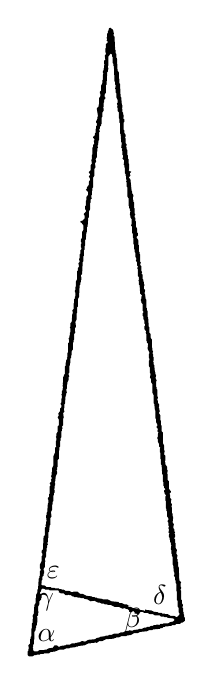
\begin{tikzpicture}[x=0.00777385cm,y=-0.00777385cm]
\fill[even odd rule] (151,17) -- (149,18) -- (148,22) -- (147,23) -- (147,26) -- (146,27) -- (146,32) -- (145,33) -- (146,36) -- (145,38) -- (147,40) -- (147,41) -- (144,44) -- (144,50) -- (143,51) -- (143,57) -- (144,58) -- (144,60) -- (142,63) -- (143,69) -- (141,71) -- (141,76) -- (142,78) -- (141,79) -- (141,83) -- (140,84) -- (140,87) -- (139,88) -- (139,91) -- (140,92) -- (139,94) -- (139,102) -- (138,103) -- (138,108) -- (136,112) -- (136,120) -- (134,122) -- (134,124) -- (135,125) -- (135,129) -- (133,132) -- (133,142) -- (132,143) -- (132,146) -- (129,149) -- (131,162) -- (130,163) -- (130,166) -- (128,170) -- (128,172) -- (129,173) -- (129,177) -- (128,178) -- (128,182) -- (127,183) -- (127,189) -- (126,190) -- (126,193) -- (124,195) -- (123,195) -- (123,197) -- (125,199) -- (125,201) -- (124,202) -- (125,206) -- (123,209) -- (123,212) -- (122,213) -- (122,224) -- (121,225) -- (121,232) -- (120,233) -- (121,239) -- (119,242) -- (119,250) -- (116,253) -- (116,254) -- (118,256) -- (118,258) -- (116,260) -- (118,264) -- (118,266) -- (116,269) -- (116,274) -- (113,278) -- (113,280) -- (111,282) -- (115,286) -- (115,290) -- (112,294) -- (112,299) -- (111,300) -- (111,308) -- (110,309) -- (110,314) -- (111,315) -- (111,318) -- (108,321) -- (108,323) -- (109,324) -- (109,329) -- (105,333) -- (103,333) -- (102,334) -- (102,335) -- (104,336) -- (107,340) -- (107,348) -- (105,351) -- (105,360) -- (103,364) -- (103,367) -- (104,368) -- (104,370) -- (103,371) -- (103,376) -- (104,377) -- (104,379) -- (102,381) -- (102,387) -- (101,388) -- (101,394) -- (100,395) -- (101,400) -- (99,402) -- (100,408) -- (98,410) -- (98,414) -- (97,415) -- (97,428) -- (95,432) -- (95,440) -- (94,441) -- (94,446) -- (93,447) -- (93,449) -- (94,450) -- (94,456) -- (93,457) -- (93,460) -- (92,461) -- (92,467) -- (91,468) -- (91,477) -- (89,479) -- (90,484) -- (89,485) -- (88,498) -- (86,500) -- (86,506) -- (85,507) -- (86,509) -- (86,515) -- (85,516) -- (85,520) -- (84,521) -- (84,524) -- (83,525) -- (84,531) -- (82,533) -- (82,548) -- (81,549) -- (81,556) -- (80,557) -- (81,558) -- (79,561) -- (79,564) -- (78,565) -- (78,570) -- (77,571) -- (77,583) -- (75,585) -- (75,587) -- (74,588) -- (74,597) -- (73,598) -- (74,600) -- (73,602) -- (74,606) -- (73,607) -- (73,610) -- (72,611) -- (72,616) -- (71,617) -- (72,619) -- (72,623) -- (71,624) -- (71,630) -- (70,631) -- (70,633) -- (71,634) -- (71,638) -- (69,640) -- (69,644) -- (66,648) -- (67,651) -- (65,654) -- (67,658) -- (67,667) -- (65,669) -- (65,678) -- (63,681) -- (63,685) -- (62,686) -- (63,688) -- (63,692) -- (62,693) -- (62,700) -- (63,702) -- (61,704) -- (61,711) -- (58,718) -- (58,733) -- (56,737) -- (56,743) -- (55,744) -- (55,749) -- (54,750) -- (55,752) -- (55,755) -- (54,756) -- (55,759) -- (52,762) -- (53,764) -- (53,766) -- (52,767) -- (52,779) -- (51,780) -- (51,784) -- (49,786) -- (49,788) -- (50,789) -- (50,794) -- (49,795) -- (48,809) -- (47,810) -- (47,814) -- (46,815) -- (47,824) -- (46,825) -- (46,829) -- (45,830) -- (46,833) -- (44,835) -- (44,847) -- (42,849) -- (41,870) -- (39,872) -- (39,876) -- (40,877) -- (40,880) -- (39,881) -- (39,889) -- (36,895) -- (36,901) -- (37,902) -- (37,905) -- (36,906) -- (36,913) -- (35,914) -- (35,917) -- (34,918) -- (33,935) -- (32,936) -- (32,940) -- (30,944) -- (30,949) -- (29,950) -- (29,958) -- (27,961) -- (26,975) -- (24,979) -- (25,983) -- (24,984) -- (24,990) -- (23,991) -- (23,999) -- (22,1000) -- (22,1012) -- (21,1013) -- (21,1016) -- (20,1017) -- (20,1024) -- (17,1027) -- (18,1032) -- (17,1033) -- (17,1036) -- (16,1037) -- (16,1043) -- (18,1045) -- (24,1045) -- (27,1043) -- (30,1043) -- (31,1042) -- (36,1042) -- (37,1041) -- (42,1041) -- (43,1040) -- (51,1040) -- (53,1038) -- (61,1037) -- (68,1034) -- (75,1034) -- (79,1032) -- (84,1032) -- (85,1031) -- (94,1030) -- (95,1029) -- (98,1029) -- (99,1028) -- (109,1027) -- (115,1024) -- (119,1024) -- (120,1023) -- (125,1023) -- (126,1022) -- (129,1023) -- (133,1020) -- (138,1020) -- (144,1017) -- (157,1016) -- (158,1015) -- (160,1015) -- (161,1014) -- (165,1014) -- (169,1012) -- (177,1012) -- (178,1011) -- (185,1010) -- (190,1007) -- (196,1007) -- (200,1005) -- (211,1004) -- (215,1002) -- (220,1002) -- (221,1001) -- (232,1000) -- (233,999) -- (236,999) -- (238,997) -- (240,997) -- (241,996) -- (246,996) -- (247,995) -- (251,995) -- (252,994) -- (257,994) -- (259,992) -- (265,992) -- (267,990) -- (269,990) -- (273,987) -- (273,982) -- (272,981) -- (272,977) -- (271,976) -- (271,973) -- (270,972) -- (270,966) -- (269,965) -- (270,961) -- (268,958) -- (268,953) -- (267,952) -- (267,938) -- (266,937) -- (266,935) -- (267,934) -- (267,932) -- (266,931) -- (266,926) -- (267,924) -- (264,921) -- (263,899) -- (262,898) -- (262,891) -- (261,890) -- (261,886) -- (260,885) -- (261,880) -- (259,877) -- (260,871) -- (258,868) -- (258,860) -- (257,859) -- (257,854) -- (256,853) -- (256,851) -- (257,850) -- (257,846) -- (256,844) -- (257,842) -- (256,841) -- (256,838) -- (254,835) -- (255,829) -- (253,826) -- (254,817) -- (253,816) -- (253,812) -- (252,811) -- (252,802) -- (251,801) -- (252,796) -- (250,794) -- (251,788) -- (249,786) -- (249,781) -- (248,780) -- (248,779) -- (250,777) -- (250,775) -- (247,771) -- (247,759) -- (245,757) -- (245,747) -- (244,746) -- (245,741) -- (244,740) -- (244,735) -- (241,731) -- (241,728) -- (240,727) -- (241,725) -- (241,717) -- (239,715) -- (240,709) -- (239,708) -- (239,700) -- (237,696) -- (237,679) -- (235,677) -- (235,668) -- (234,667) -- (234,660) -- (233,659) -- (233,651) -- (231,648) -- (231,646) -- (232,645) -- (231,639) -- (230,638) -- (231,636) -- (231,633) -- (229,631) -- (229,627) -- (228,626) -- (228,624) -- (229,623) -- (229,621) -- (228,620) -- (228,609) -- (227,608) -- (227,605) -- (226,604) -- (226,596) -- (227,594) -- (225,590) -- (226,585) -- (225,584) -- (225,581) -- (224,580) -- (223,569) -- (222,568) -- (222,564) -- (221,563) -- (222,561) -- (222,556) -- (221,555) -- (221,551) -- (220,550) -- (221,546) -- (220,545) -- (220,541) -- (219,540) -- (219,527) -- (217,524) -- (217,518) -- (215,516) -- (215,507) -- (214,506) -- (213,491) -- (212,490) -- (212,480) -- (211,479) -- (211,476) -- (210,475) -- (210,462) -- (209,461) -- (208,453) -- (207,452) -- (208,446) -- (206,444) -- (206,440) -- (207,439) -- (207,437) -- (206,436) -- (206,433) -- (205,432) -- (205,429) -- (204,428) -- (204,421) -- (202,419) -- (203,417) -- (202,415) -- (202,407) -- (200,405) -- (201,401) -- (200,400) -- (200,388) -- (199,387) -- (199,384) -- (198,383) -- (198,373) -- (197,372) -- (197,365) -- (194,360) -- (194,359) -- (196,357) -- (196,353) -- (195,352) -- (195,346) -- (193,342) -- (193,334) -- (192,333) -- (192,328) -- (191,327) -- (191,324) -- (192,322) -- (191,321) -- (191,313) -- (190,312) -- (190,303) -- (189,302) -- (189,299) -- (188,298) -- (188,294) -- (189,293) -- (189,291) -- (187,288) -- (187,285) -- (186,284) -- (184,265) -- (182,263) -- (182,261) -- (184,259) -- (183,255) -- (185,253) -- (185,252) -- (183,252) -- (181,250) -- (182,248) -- (182,240) -- (181,239) -- (181,232) -- (180,231) -- (180,226) -- (179,225) -- (179,217) -- (178,216) -- (178,213) -- (177,212) -- (178,208) -- (176,206) -- (176,198) -- (175,197) -- (176,195) -- (176,192) -- (174,189) -- (174,185) -- (173,184) -- (173,172) -- (174,171) -- (174,167) -- (172,165) -- (173,163) -- (173,160) -- (172,159) -- (172,156) -- (171,155) -- (171,150) -- (170,149) -- (171,147) -- (171,144) -- (170,143) -- (169,131) -- (168,130) -- (167,109) -- (166,108) -- (166,101) -- (165,100) -- (165,90) -- (163,87) -- (162,67) -- (161,66) -- (161,60) -- (160,59) -- (160,54) -- (159,53) -- (158,32) -- (156,29) -- (157,27) -- (156,22) -- (155,20) -- cycle
(24,1031) -- (25,1029) -- (25,1026) -- (26,1025) -- (26,1018) -- (27,1017) -- (27,1005) -- (29,1002) -- (29,999) -- (30,998) -- (30,995) -- (31,994) -- (31,990) -- (32,989) -- (32,982) -- (31,980) -- (33,978) -- (33,974) -- (34,973) -- (33,971) -- (33,964) -- (35,960) -- (35,955) -- (38,952) -- (38,950) -- (39,949) -- (39,944) -- (40,943) -- (38,944) -- (36,942) -- (36,941) -- (38,938) -- (38,936) -- (40,934) -- (44,935) -- (45,936) -- (51,936) -- (52,937) -- (66,937) -- (67,938) -- (67,941) -- (69,941) -- (70,942) -- (75,942) -- (78,945) -- (81,945) -- (83,944) -- (84,945) -- (87,945) -- (89,947) -- (91,947) -- (92,948) -- (97,948) -- (98,949) -- (102,949) -- (103,950) -- (108,950) -- (109,951) -- (114,952) -- (119,955) -- (125,954) -- (131,957) -- (134,957) -- (137,959) -- (141,959) -- (142,960) -- (146,960) -- (147,961) -- (152,961) -- (158,964) -- (165,964) -- (171,967) -- (175,966) -- (176,967) -- (180,968) -- (182,970) -- (182,972) -- (186,973) -- (188,971) -- (189,971) -- (191,973) -- (191,975) -- (194,975) -- (195,976) -- (196,976) -- (199,973) -- (203,972) -- (207,974) -- (212,974) -- (216,976) -- (221,976) -- (224,978) -- (232,978) -- (234,980) -- (239,980) -- (240,981) -- (244,981) -- (245,982) -- (254,983) -- (256,985) -- (256,986) -- (254,988) -- (249,989) -- (246,991) -- (238,991) -- (237,992) -- (233,992) -- (231,994) -- (229,993) -- (227,993) -- (226,994) -- (222,994) -- (221,995) -- (218,995) -- (215,997) -- (211,997) -- (210,998) -- (207,998) -- (203,1000) -- (198,1000) -- (197,1001) -- (189,1002) -- (188,1003) -- (184,1003) -- (183,1002) -- (182,1003) -- (175,1004) -- (172,1006) -- (168,1006) -- (164,1008) -- (157,1008) -- (153,1010) -- (149,1010) -- (148,1011) -- (144,1011) -- (143,1012) -- (135,1013) -- (134,1014) -- (129,1015) -- (126,1017) -- (115,1018) -- (110,1021) -- (105,1020) -- (101,1022) -- (98,1022) -- (97,1023) -- (94,1023) -- (93,1024) -- (88,1024) -- (85,1026) -- (79,1026) -- (78,1027) -- (70,1028) -- (69,1029) -- (66,1029) -- (64,1027) -- (60,1027) -- (57,1031) -- (50,1032) -- (47,1034) -- (44,1034) -- (43,1035) -- (35,1035) -- (32,1037) -- (27,1037) -- (25,1035) -- (25,1032) -- cycle
(152,59) -- (154,61) -- (154,64) -- (155,65) -- (155,75) -- (156,76) -- (156,79) -- (157,80) -- (158,105) -- (159,106) -- (159,110) -- (160,111) -- (159,117) -- (160,118) -- (160,123) -- (161,124) -- (161,131) -- (163,135) -- (163,140) -- (162,141) -- (163,145) -- (162,147) -- (163,148) -- (163,153) -- (165,155) -- (165,165) -- (166,166) -- (166,172) -- (167,173) -- (167,190) -- (168,191) -- (169,204) -- (170,205) -- (169,213) -- (171,215) -- (170,217) -- (171,219) -- (171,225) -- (172,226) -- (172,229) -- (171,231) -- (174,234) -- (173,241) -- (174,242) -- (174,245) -- (175,246) -- (175,255) -- (176,256) -- (176,259) -- (177,260) -- (177,265) -- (178,266) -- (177,269) -- (178,270) -- (178,277) -- (179,278) -- (179,293) -- (181,296) -- (181,308) -- (182,309) -- (182,312) -- (183,313) -- (183,316) -- (184,317) -- (183,323) -- (184,324) -- (184,327) -- (186,330) -- (186,338) -- (185,340) -- (187,343) -- (187,353) -- (188,354) -- (188,360) -- (189,361) -- (189,371) -- (190,372) -- (190,379) -- (191,380) -- (191,384) -- (192,385) -- (192,391) -- (194,395) -- (193,398) -- (195,401) -- (195,406) -- (196,407) -- (196,409) -- (195,410) -- (196,412) -- (196,423) -- (198,425) -- (198,429) -- (197,431) -- (198,432) -- (198,437) -- (199,438) -- (200,452) -- (203,455) -- (202,457) -- (202,460) -- (201,461) -- (201,464) -- (202,465) -- (202,467) -- (204,469) -- (204,480) -- (205,481) -- (205,483) -- (204,484) -- (204,488) -- (205,489) -- (205,493) -- (207,496) -- (207,501) -- (208,502) -- (208,504) -- (207,505) -- (207,510) -- (210,514) -- (209,516) -- (210,518) -- (210,529) -- (211,530) -- (211,532) -- (213,534) -- (212,542) -- (215,548) -- (215,550) -- (214,551) -- (214,557) -- (215,558) -- (215,561) -- (214,562) -- (214,570) -- (216,573) -- (216,582) -- (217,583) -- (216,589) -- (218,592) -- (218,597) -- (220,600) -- (220,614) -- (222,618) -- (222,631) -- (223,632) -- (224,642) -- (225,643) -- (225,656) -- (226,657) -- (226,662) -- (228,666) -- (228,668) -- (227,669) -- (227,671) -- (229,673) -- (228,677) -- (230,679) -- (229,681) -- (229,686) -- (228,687) -- (228,689) -- (229,690) -- (229,694) -- (231,698) -- (231,702) -- (233,704) -- (232,706) -- (232,711) -- (233,712) -- (233,722) -- (234,723) -- (234,731) -- (235,732) -- (236,747) -- (237,748) -- (237,759) -- (238,760) -- (238,766) -- (239,767) -- (239,769) -- (241,771) -- (241,772) -- (239,774) -- (239,776) -- (240,777) -- (240,779) -- (242,781) -- (242,783) -- (241,784) -- (241,790) -- (242,791) -- (242,803) -- (243,804) -- (243,807) -- (244,808) -- (244,816) -- (246,819) -- (246,822) -- (245,823) -- (245,825) -- (246,826) -- (246,831) -- (247,832) -- (247,834) -- (246,835) -- (247,837) -- (247,840) -- (246,842) -- (248,844) -- (247,846) -- (247,850) -- (248,851) -- (248,854) -- (249,855) -- (249,858) -- (250,859) -- (250,862) -- (251,863) -- (250,870) -- (251,871) -- (251,877) -- (252,878) -- (252,881) -- (253,882) -- (253,895) -- (254,896) -- (255,907) -- (256,908) -- (256,911) -- (255,913) -- (257,916) -- (257,920) -- (258,921) -- (258,925) -- (259,926) -- (259,938) -- (260,939) -- (260,953) -- (261,954) -- (261,963) -- (263,966) -- (263,973) -- (264,974) -- (264,977) -- (260,981) -- (256,979) -- (250,979) -- (245,976) -- (241,976) -- (240,975) -- (236,975) -- (235,974) -- (230,974) -- (229,973) -- (222,972) -- (218,970) -- (209,969) -- (208,968) -- (208,970) -- (207,971) -- (206,970) -- (199,969) -- (195,967) -- (188,966) -- (184,964) -- (181,964) -- (180,963) -- (181,962) -- (184,962) -- (181,962) -- (178,960) -- (174,960) -- (170,958) -- (166,958) -- (164,956) -- (153,955) -- (147,952) -- (139,952) -- (138,951) -- (130,950) -- (129,949) -- (126,949) -- (125,948) -- (122,948) -- (121,947) -- (112,946) -- (106,943) -- (102,943) -- (97,939) -- (91,939) -- (90,940) -- (88,940) -- (84,938) -- (78,938) -- (75,936) -- (72,936) -- (71,935) -- (68,935) -- (67,934) -- (61,934) -- (60,933) -- (55,933) -- (54,932) -- (47,932) -- (45,930) -- (43,929) -- (40,929) -- (38,927) -- (39,925) -- (39,921) -- (40,920) -- (40,915) -- (42,913) -- (42,910) -- (43,909) -- (43,905) -- (42,904) -- (42,902) -- (44,899) -- (44,891) -- (45,890) -- (44,886) -- (46,882) -- (46,874) -- (47,873) -- (47,868) -- (48,867) -- (48,863) -- (49,862) -- (48,859) -- (49,858) -- (49,852) -- (50,851) -- (50,842) -- (51,841) -- (52,831) -- (53,830) -- (53,819) -- (55,816) -- (54,809) -- (56,805) -- (56,797) -- (57,796) -- (57,792) -- (58,791) -- (58,782) -- (59,781) -- (59,778) -- (60,777) -- (60,773) -- (59,772) -- (60,770) -- (60,766) -- (61,765) -- (61,762) -- (60,760) -- (61,759) -- (62,750) -- (64,746) -- (64,743) -- (63,741) -- (64,740) -- (64,736) -- (65,735) -- (65,724) -- (67,722) -- (67,709) -- (68,708) -- (68,703) -- (69,702) -- (69,693) -- (70,692) -- (70,688) -- (71,687) -- (71,677) -- (72,676) -- (72,673) -- (73,672) -- (72,669) -- (74,667) -- (74,656) -- (75,655) -- (74,647) -- (76,645) -- (75,640) -- (76,639) -- (76,633) -- (77,632) -- (78,619) -- (79,618) -- (79,615) -- (80,614) -- (79,608) -- (80,607) -- (80,601) -- (81,600) -- (81,597) -- (83,593) -- (83,588) -- (84,587) -- (83,585) -- (83,582) -- (84,581) -- (84,570) -- (85,569) -- (85,566) -- (86,565) -- (86,558) -- (87,557) -- (87,553) -- (88,552) -- (88,546) -- (90,543) -- (90,532) -- (91,531) -- (91,528) -- (92,527) -- (92,518) -- (94,515) -- (93,513) -- (93,509) -- (95,506) -- (94,498) -- (96,494) -- (96,484) -- (97,483) -- (97,474) -- (98,473) -- (98,461) -- (100,457) -- (101,438) -- (102,437) -- (102,434) -- (103,433) -- (103,430) -- (104,429) -- (104,425) -- (103,424) -- (103,422) -- (105,420) -- (106,400) -- (107,399) -- (107,391) -- (108,390) -- (108,381) -- (109,380) -- (109,374) -- (110,373) -- (110,364) -- (111,363) -- (112,352) -- (113,351) -- (113,343) -- (114,342) -- (115,328) -- (116,327) -- (116,318) -- (118,314) -- (118,304) -- (119,303) -- (119,298) -- (121,296) -- (120,294) -- (120,291) -- (121,290) -- (121,284) -- (122,283) -- (122,279) -- (123,278) -- (123,262) -- (125,259) -- (125,248) -- (127,245) -- (126,239) -- (128,236) -- (127,232) -- (129,229) -- (129,220) -- (130,219) -- (130,214) -- (131,213) -- (130,210) -- (131,209) -- (132,201) -- (133,200) -- (133,188) -- (134,187) -- (133,183) -- (134,182) -- (134,179) -- (136,177) -- (136,175) -- (137,174) -- (137,164) -- (138,163) -- (138,156) -- (140,153) -- (140,149) -- (139,148) -- (140,147) -- (140,140) -- (141,139) -- (141,135) -- (143,133) -- (143,131) -- (142,130) -- (142,126) -- (144,123) -- (144,111) -- (145,110) -- (146,90) -- (147,89) -- (147,86) -- (148,85) -- (148,83) -- (147,82) -- (147,80) -- (148,79) -- (148,64) -- cycle;
\node[inner sep=0pt] at (58,908) {$\varepsilon$};
\node[inner sep=0pt] at (232,944) {$\delta$};
\node[inner sep=0pt] at (46,957) {$\gamma$};
\node[inner sep=0pt] at (188,987) {$\beta$};
\node[inner sep=0pt] at (47,1011) {$\alpha$};
\end{tikzpicture}

\end{minipage}\hfill\begin{minipage}[t]{9.9cm}\vspace{0pt}

 Das Übrige ergibt sich dann leicht von selbst. Es ist nemlich nach diesem Lehrsatze

\[
\alpha+\beta+\delta=180^0
\]
\[
180^0=\varepsilon+\delta
\]
\[
\gamma+\varepsilon=180^0.
\]

 Also addendo

\[
\alpha+\beta+\gamma=180^0.
\]

 \end{minipage}

Was nun aber Ihren Beweis für 1) betrifft, so protestire ich zuvörderst gegen den Gebrauch einer unendlichen Grösse als einer \textls{Vollendeten}, welcher in der Mathematik niemals erlaubt ist. Das Unendliche ist nur eine façon de parler, indem man eigentlich von Grenzen spricht, denen gewisse Verhältnisse so nahe kommen als man will, während andern ohne Einschränkung zu wachsen verstattet ist. In diesem Sinne enthält die Nicht-Euklidische Geometrie durchaus nichts widersprechendes, wenn gleich diejenigen[, die sie kennen lernen,] viele Ergebnisse derselben anfangs für paradox halten müssen, was aber für widersprechend zu halten nur eine Selbsttäuschung sein würde, hervorgebracht von der frühen Gewöhnung, die Euklidische Geometrie für \textls{streng} wahr zu halten.

In der Nicht-Euklidischen Geometrie gibt es gar keine ähnlichen Figuren ohne Gleichheit, z.\,B. die Winkel eines gleichseitigen Dreiecks sind nicht bloss von $\frac{2}{3}R$, sondern auch [bei verschiedenem Dreiecken] nach Massgabe der Grösse der Seiten unter sich verschieden und können, wenn die Seite über alle Grenzen wächst, so klein werden, wie man will. Es ist daher schon an sich widersprechend, ein solches Dreieck durch ein kleineres \textls{zeichnen} zu wollen, man kann es im Grunde nur \textls{bezeichnen}:

\begin{center}
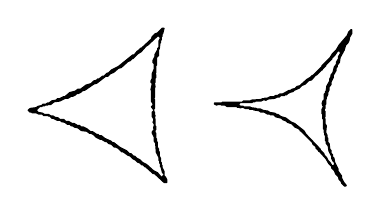
\begin{tikzpicture}[x=0.00869565cm,y=-0.00869565cm]
\fill[even odd rule] (493,13) -- (492,13) -- (488,17) -- (486,22) -- (474,36) -- (470,43) -- (464,49) -- (461,54) -- (449,66) -- (449,67) -- (436,80) -- (435,80) -- (432,83) -- (427,86) -- (417,95) -- (413,96) -- (410,99) -- (406,100) -- (403,102) -- (401,102) -- (392,107) -- (388,107) -- (385,109) -- (382,109) -- (379,111) -- (374,111) -- (370,113) -- (366,113) -- (365,114) -- (362,114) -- (361,115) -- (346,116) -- (345,117) -- (335,117) -- (333,119) -- (304,119) -- (303,120) -- (293,120) -- (292,121) -- (292,123) -- (296,125) -- (298,124) -- (302,124) -- (303,125) -- (308,125) -- (311,127) -- (325,127) -- (326,128) -- (329,128) -- (330,129) -- (334,128) -- (338,130) -- (343,130) -- (344,131) -- (349,131) -- (350,132) -- (357,133) -- (360,135) -- (365,135) -- (370,138) -- (373,138) -- (374,139) -- (379,139) -- (382,142) -- (390,144) -- (392,146) -- (397,148) -- (399,150) -- (405,152) -- (410,157) -- (415,159) -- (417,161) -- (417,162) -- (419,163) -- (435,179) -- (436,182) -- (440,185) -- (440,187) -- (444,191) -- (444,192) -- (446,193) -- (455,203) -- (459,210) -- (463,214) -- (463,216) -- (467,220) -- (469,225) -- (473,229) -- (474,233) -- (477,236) -- (478,239) -- (482,243) -- (485,243) -- (486,241) -- (482,236) -- (479,230) -- (479,227) -- (474,220) -- (474,217) -- (469,207) -- (468,201) -- (466,199) -- (466,196) -- (464,194) -- (464,190) -- (462,188) -- (461,180) -- (459,178) -- (459,172) -- (458,171) -- (458,168) -- (456,164) -- (457,154) -- (455,151) -- (455,144) -- (454,143) -- (455,141) -- (455,133) -- (454,132) -- (454,130) -- (455,129) -- (455,124) -- (456,123) -- (456,116) -- (457,115) -- (457,113) -- (459,109) -- (459,106) -- (461,102) -- (461,98) -- (464,94) -- (464,90) -- (467,84) -- (467,81) -- (471,74) -- (471,71) -- (473,68) -- (473,66) -- (476,62) -- (477,55) -- (483,44) -- (485,37) -- (488,34) -- (490,30) -- (491,25) -- (494,20) -- (494,14) -- cycle
(475,46) -- (476,48) -- (473,53) -- (473,56) -- (470,61) -- (470,64) -- (467,68) -- (465,76) -- (462,80) -- (462,82) -- (460,86) -- (460,89) -- (456,96) -- (455,103) -- (454,104) -- (454,106) -- (452,108) -- (452,116) -- (450,118) -- (450,120) -- (449,121) -- (450,125) -- (451,126) -- (449,130) -- (449,137) -- (450,138) -- (450,144) -- (451,145) -- (451,159) -- (452,160) -- (452,164) -- (453,165) -- (453,168) -- (454,169) -- (454,176) -- (455,177) -- (455,180) -- (458,184) -- (459,191) -- (463,199) -- (463,202) -- (465,206) -- (467,208) -- (467,211) -- (465,212) -- (462,207) -- (459,204) -- (457,200) -- (454,197) -- (453,194) -- (448,189) -- (448,188) -- (427,166) -- (424,161) -- (410,150) -- (405,148) -- (397,142) -- (390,140) -- (386,137) -- (384,137) -- (381,135) -- (374,134) -- (371,132) -- (364,131) -- (360,129) -- (355,129) -- (354,128) -- (346,127) -- (345,126) -- (336,126) -- (335,125) -- (331,125) -- (329,123) -- (331,121) -- (348,121) -- (349,120) -- (352,120) -- (353,119) -- (361,119) -- (365,117) -- (368,118) -- (371,116) -- (381,115) -- (385,113) -- (388,113) -- (390,111) -- (395,111) -- (396,110) -- (398,110) -- (400,108) -- (404,106) -- (408,105) -- (410,103) -- (417,100) -- (421,96) -- (426,94) -- (431,89) -- (435,88) -- (441,81) -- (442,81) -- (449,74) -- (451,73) -- (451,72) -- (456,67) -- (456,66) -- (465,57) -- (465,56) -- (469,52) -- (473,46) -- cycle
(220,12) -- (219,11) -- (216,11) -- (209,18) -- (206,19) -- (201,24) -- (200,27) -- (186,40) -- (185,40) -- (181,44) -- (180,44) -- (175,50) -- (173,50) -- (152,67) -- (142,72) -- (138,76) -- (135,77) -- (131,81) -- (129,81) -- (124,85) -- (122,85) -- (120,87) -- (116,88) -- (112,92) -- (105,94) -- (97,100) -- (93,100) -- (89,103) -- (81,105) -- (74,111) -- (72,111) -- (66,114) -- (63,114) -- (61,116) -- (55,117) -- (51,120) -- (49,120) -- (46,122) -- (42,122) -- (40,124) -- (35,125) -- (32,127) -- (24,128) -- (22,129) -- (20,131) -- (20,132) -- (23,135) -- (25,135) -- (26,136) -- (32,136) -- (36,138) -- (41,138) -- (43,140) -- (49,140) -- (50,141) -- (52,141) -- (55,144) -- (57,144) -- (63,147) -- (67,147) -- (69,149) -- (74,150) -- (78,153) -- (81,153) -- (83,155) -- (85,155) -- (88,157) -- (93,158) -- (98,162) -- (106,163) -- (110,166) -- (112,166) -- (116,168) -- (120,172) -- (126,175) -- (128,175) -- (133,178) -- (135,178) -- (138,181) -- (142,182) -- (146,186) -- (148,186) -- (152,188) -- (157,193) -- (159,193) -- (166,198) -- (169,199) -- (173,203) -- (177,205) -- (180,208) -- (183,209) -- (186,212) -- (188,212) -- (191,215) -- (192,215) -- (203,225) -- (205,225) -- (219,238) -- (223,238) -- (224,237) -- (224,233) -- (222,229) -- (220,227) -- (220,221) -- (217,215) -- (217,212) -- (216,211) -- (216,208) -- (215,207) -- (215,202) -- (213,198) -- (213,192) -- (212,191) -- (212,188) -- (210,185) -- (210,178) -- (209,177) -- (209,173) -- (208,172) -- (208,165) -- (207,164) -- (207,161) -- (208,160) -- (208,155) -- (207,154) -- (207,144) -- (206,143) -- (207,139) -- (206,138) -- (206,134) -- (205,133) -- (205,130) -- (206,129) -- (206,116) -- (205,114) -- (206,113) -- (206,99) -- (207,98) -- (206,92) -- (207,91) -- (207,85) -- (208,84) -- (208,80) -- (207,78) -- (208,77) -- (208,67) -- (209,66) -- (209,55) -- (212,52) -- (212,43) -- (213,42) -- (214,34) -- (215,33) -- (215,30) -- (216,29) -- (216,25) -- (217,24) -- (217,21) -- (218,20) -- cycle
(213,26) -- (211,30) -- (211,39) -- (209,41) -- (209,43) -- (205,50) -- (205,53) -- (202,59) -- (202,62) -- (204,64) -- (204,71) -- (201,78) -- (201,85) -- (199,89) -- (199,91) -- (201,93) -- (199,102) -- (200,103) -- (200,119) -- (202,122) -- (202,124) -- (200,126) -- (200,127) -- (203,131) -- (203,132) -- (201,134) -- (201,141) -- (203,144) -- (203,147) -- (202,149) -- (204,152) -- (204,155) -- (203,156) -- (203,158) -- (204,159) -- (201,163) -- (201,165) -- (204,171) -- (204,177) -- (206,180) -- (207,193) -- (211,201) -- (211,205) -- (212,206) -- (212,209) -- (213,210) -- (213,214) -- (214,215) -- (216,223) -- (218,225) -- (218,226) -- (216,228) -- (215,228) -- (210,222) -- (204,219) -- (194,210) -- (188,207) -- (184,203) -- (180,201) -- (177,198) -- (175,198) -- (171,194) -- (169,194) -- (165,190) -- (155,185) -- (146,178) -- (144,178) -- (142,176) -- (133,172) -- (128,168) -- (125,168) -- (123,166) -- (121,166) -- (115,162) -- (112,162) -- (107,158) -- (101,155) -- (98,155) -- (96,153) -- (93,153) -- (88,150) -- (85,150) -- (80,147) -- (76,147) -- (73,144) -- (67,144) -- (65,142) -- (60,141) -- (57,139) -- (54,139) -- (51,137) -- (45,137) -- (42,135) -- (36,134) -- (34,132) -- (34,131) -- (38,127) -- (41,127) -- (42,126) -- (45,126) -- (46,125) -- (49,125) -- (50,124) -- (54,124) -- (59,120) -- (67,119) -- (75,115) -- (79,115) -- (84,112) -- (86,112) -- (90,110) -- (92,108) -- (94,108) -- (98,106) -- (100,104) -- (104,103) -- (117,94) -- (121,93) -- (134,83) -- (137,83) -- (141,79) -- (146,77) -- (153,71) -- (157,70) -- (167,61) -- (170,60) -- (173,57) -- (174,57) -- (181,50) -- (186,47) -- (194,38) -- (195,38) -- (210,24) -- (211,24) -- cycle;
\end{tikzpicture}

\end{center}

 Die Bezeichnung des unendlichen Dreiecks in diesem Sinne wäre am Ende:

\begin{center}
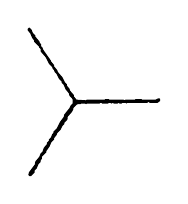
\begin{tikzpicture}[x=0.00816327cm,y=-0.00816327cm]
\fill[even odd rule] (14,239) -- (16,241) -- (18,241) -- (24,235) -- (24,232) -- (27,229) -- (30,222) -- (33,219) -- (33,217) -- (35,214) -- (35,211) -- (42,204) -- (42,202) -- (47,195) -- (50,188) -- (54,184) -- (54,182) -- (58,177) -- (59,174) -- (64,169) -- (67,163) -- (70,160) -- (70,158) -- (74,154) -- (75,152) -- (75,149) -- (82,141) -- (84,137) -- (84,135) -- (89,130) -- (91,129) -- (95,129) -- (96,128) -- (102,128) -- (104,129) -- (105,128) -- (125,128) -- (126,127) -- (128,127) -- (129,128) -- (138,128) -- (139,127) -- (142,127) -- (143,128) -- (145,127) -- (147,128) -- (153,128) -- (154,127) -- (156,128) -- (159,128) -- (160,127) -- (165,127) -- (167,128) -- (168,127) -- (199,127) -- (200,126) -- (202,126) -- (203,127) -- (215,127) -- (219,124) -- (219,121) -- (218,120) -- (216,120) -- (212,122) -- (191,122) -- (190,121) -- (181,121) -- (180,122) -- (165,122) -- (164,123) -- (162,122) -- (140,122) -- (139,121) -- (134,121) -- (133,122) -- (105,122) -- (104,123) -- (89,122) -- (85,117) -- (85,115) -- (79,108) -- (78,105) -- (74,100) -- (74,98) -- (71,95) -- (67,87) -- (60,79) -- (59,76) -- (54,70) -- (54,68) -- (49,62) -- (49,61) -- (37,44) -- (36,41) -- (34,39) -- (34,36) -- (32,34) -- (31,31) -- (25,24) -- (25,22) -- (21,18) -- (19,13) -- (16,10) -- (15,10) -- (13,12) -- (13,14) -- (17,19) -- (20,26) -- (23,30) -- (23,32) -- (31,40) -- (31,41) -- (33,43) -- (33,46) -- (34,48) -- (41,56) -- (46,66) -- (51,71) -- (52,74) -- (54,76) -- (55,79) -- (58,82) -- (62,90) -- (66,94) -- (66,96) -- (69,99) -- (72,106) -- (77,112) -- (78,116) -- (82,120) -- (83,122) -- (83,128) -- (80,131) -- (78,135) -- (70,145) -- (69,149) -- (63,157) -- (58,167) -- (53,172) -- (53,174) -- (51,176) -- (49,181) -- (46,184) -- (46,186) -- (43,189) -- (43,191) -- (38,197) -- (36,203) -- (33,206) -- (31,211) -- (25,218) -- (24,223) -- (15,235) -- cycle;
\end{tikzpicture}

\end{center}
